%Time series forecasting plays a crucial role in numerous applications, including energy, healthcare, and climate modeling, where predicting future values based on historical data can drive critical decisions. In the decision process, Uncertainty Quantification (UQ) plays a pivotal role as it allows us to estimate the confidence of our predictions, and reason about potential outcomes in a systematic manner. 


Uncertainty Quantification (UQ) is a key building block of reliable machine learning systems. Conformal prediction (CP) is a popular distribution-free UQ method that provides finite sample coverage guarantees without placing assumptions on the underlying data generating process \citep{vovk2005algorithmic, lei2018distribution}. Because of its simplicity and generality, conformal prediction has seen wide adoption in many tasks, ranging from  healthcare \cite{angelopoulos2022conformal},  robotics \cite{lindemann2023safe}, to validating the factuality of  generative models \cite{cherian2024large}.

Existing CP algorithms for time series forecasting mostly adopt an online learning framework \cite{gibbs2024conformal, angelopoulos2024pid}, where the prediction interval adapts to distribution changes in data \textit{reactively}. The online CP algorithms achieve a asymptotic marginal coverage guarantee (the miscoverage rate converges to a specified fraction as the time horizon goes to infinity). As a result, the algorithms inevitably exhibit miscoverage when distribution shifts occur, and then have to over- or under-cover in later timesteps to compensate. This behavior is evident in the ACI and CP baselines in Figure \ref{fig:cov}. This is undesirable in practice as these under-covered periods may incur a lot of risk.

This paper builds upon the observation that in real-world scenarios, distribution shifts in time-series are often \textit{predictable}. Take for example the task of forecasting electricity demands: we know that the hidden dynamics may differ between day and night, or during weekdays and weekends. The same logic applies to traffic forecasting and product demand forecasting, where there are patterns in the shifts between ``surge times" and ``normal times". In this work, we study time series data that exhibit this type of abrupt shifts, or change points, in the underlying generative process. 

State Space Models (SSMs) \citep{kalman1960new, aoki2013state} are a powerful tool for modeling time series data, as they provide a structured framework to capture the underlying temporal dependencies through latent states. In particular, Switching Dynamical Systems (SDS) \citep{ackerson1970state} is a type of SSM with an additional set of latent variables (known as \textit{switches}) that represent the operating mode active at the current timestep. SDS introduces the inductive biases that allow SSMs to switch between a discrete set of dynamics, which can be learned from training data. It is shown to be a flexible, robust, and interpretable representation of time series with varying dynamics exhibiting change points \citep{ansari2021deep, chen2022learning}. SDS is deployed not only for energy \cite{karakatsani2008intra, song2014short, fan2008machine} and traffic \cite{yu2004switching, cetin2006short} forecasting as  examples given above, but also on a wide range of applications including neuroscience \cite{glaser2020recurrent, rabinovich2006dynamical, kato2015global}, engineering \cite{strachan2011measuring,wang2007actively}, and sports analytics \cite{yamamoto2018switching}, all would benefit from robust and calibrated uncertainty quantification. 

Our code is open source at \url{https://github.com/huiwenn/CPTC}. Our contributions are:

%\begin{wrapfigure}{r}{0.5\textwidth}
\begin{figure}[tb]
    \vspace{-1em}
    \centering
    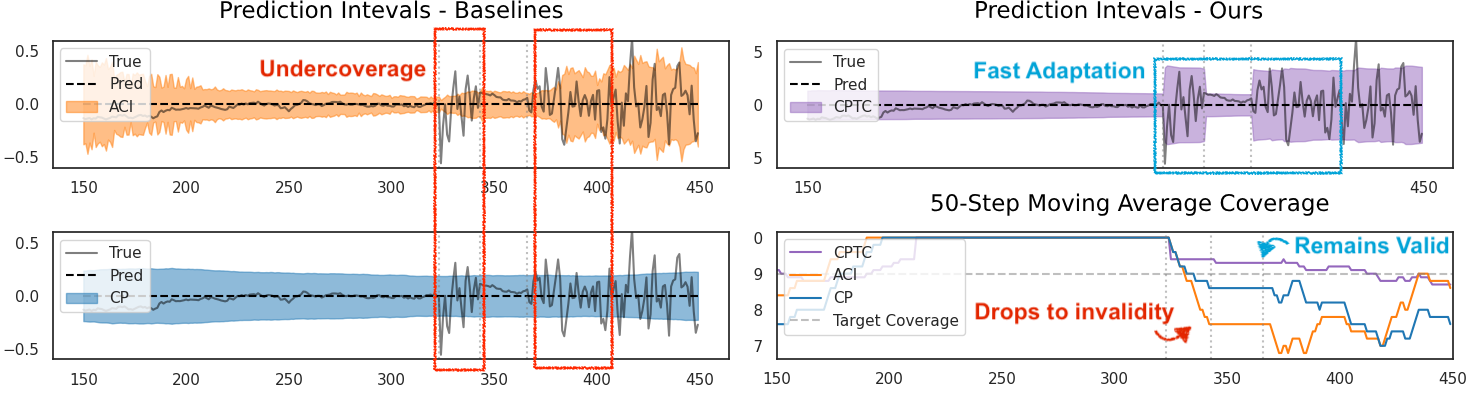
\includegraphics[width=1.01\linewidth]{changepoints/figs/ex/ex_zoom.png}
    \caption{Comparison of the prediction intervals obtained by our algorithm CPTC (purple) against online conformal prediction baselines on synthetic data. The vertical dashed line marks the distribution shifts; ideal behavior is consistent coverage at the horizontal dashed line in the final panel. Bottom right panel shows that CPTC achieves fast adaptation and remains valid when change points occur.}
    \label{fig:cov}
    \vspace{-1em}

\end{figure}
%    \vspace{-2.0em}
%\end{wrapfigure}

%
\vspace{-0.5em}
\begin{itemize}
    \item We propose a new algorithm \textbf{C}onformal \textbf{P}rediction for \textbf{T}ime series with \textbf{C}hange points (CPTC) that utilizes state transition predictions to improve uncertainty quantification for time-series forecasts. Leveraging properties of a SDS model, CPTC consolidates multiple future forecasts to adaptively adjust its prediction intervals when underlying dynamics shift.
    \item We prove that CPTC achieves asymptotic valid coverage, \textit{without assumptions} on the data generation process or state transition model accuracy. When predicted state transitions align well with distribution shifts, CPTC can anticipate uncertainty and adapt faster.
    \item We show strong empirical results on 3 synthetic and 3 real-world datasets. Compared to online conformal prediction baselines, CPTC achieves more robust coverage with comparable prediction intervals sharpness (example in Figure \ref{fig:cov}), and is computationally light.%Compared to  CP algorithms leveraging temporal structures (SPCI \cite{xu2023sequential} and HopCPT \cite{auer2023hopcpt}), CPTC is computationally lighter and more data-efficient.
\end{itemize}

%Conformal prediction produces a $(1-\alpha)$-prediction interval $\Gamma^{1-\alpha}$ for a random variable $y$, which is \textit{valid} if it contains $y$'s true value with high probability:  
%$
%\Prob[y \in \Gamma^{1-\alpha}] \geq 1-\alpha.
%$
%Note that one can make the prediction interval infinitely large to satisfy validity. But for the prediction interval to be useful, we also want to minimize its area while remaining valid; this is known as the \textit{sharpness} of the region. 


% \begin{figure}[h]
%     \centering
%     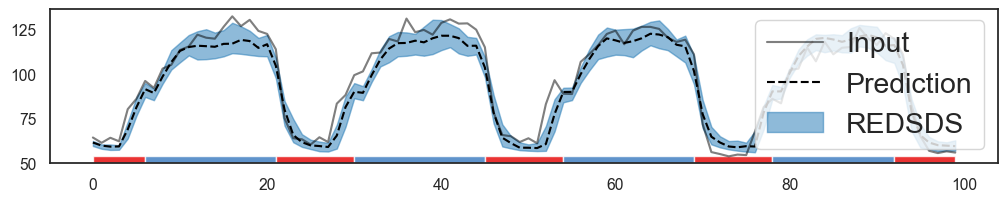
\includegraphics[width=0.9\linewidth]{changepoints/figs/e-prob.png}
%     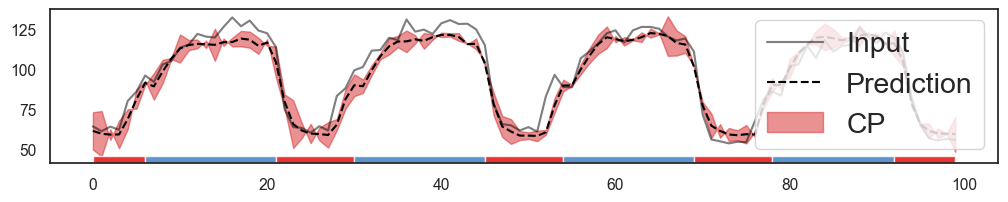
\includegraphics[width=0.9\linewidth]{changepoints/figs/e-cp.png}
%         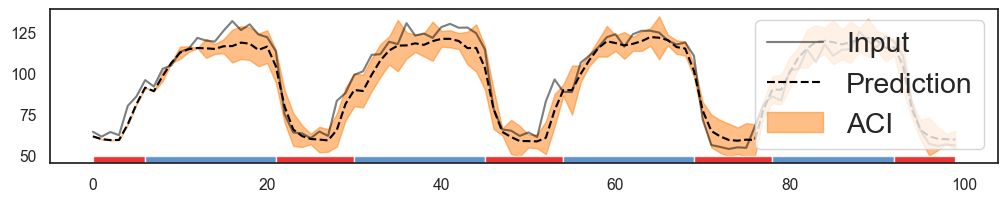
\includegraphics[width=0.9\linewidth]{changepoints/figs/e-aci.png}
%     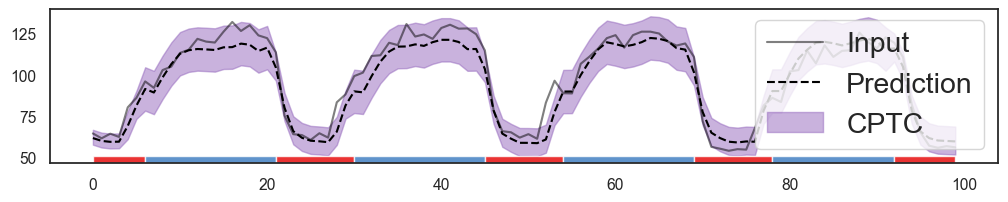
\includegraphics[width=0.9\linewidth]{changepoints/figs/e-ours.png}
%     \caption{Demonstration of uncertainty quantification baselines on hourly electricity demand. Our method (green regions) adapts to different levels of volatility between day and night and whereby achieves more stable coverage over time, whereas ACI (yellow) over-covers during red phases and under-covers during blue.}
%     \label{fig:demonstration}
% \end{figure}
